\chapter{The \textsc{go-mutesting} Framework}
\label{chapter:goMutesting}

This chapter presents \textsc{go-mutesting}, a framework for performing mutation testing on source code of the programming language \textsc{Go}. Its main purpose is to find source code, which is not covered by any tests. The implementation of \textsc{go-mutesting} with all its assets has been open sourced and is freely available at~\cite{2017_go-mutesting_repository}.

\section{Motivation}
\label{sec:goMutestingMotivation}

The generation of test suites for existing software systems is a major use case of \textsc{Tavor}. One way of evaluating the quality of these test suites is to use mutation testing~\cite{jia2011analysis}, i.e., the software under test gets modified and the generated test suite is verified by checking whether at least one test case fails and therefore if it catches the modifications. A more thorough description of mutation testing can be found in Section~\ref{sec:whatIsMutatinTesting}.

At the time of implementation of \textsc{Tavor}, there has not been any adequate mutation testing tool for the programming language \textsc{Go}. All three existing tools \textsc{manbearpig}~\cite{2017_manbearpig_repository}, \textsc{mutator}~\cite{2017_mutator_repository} and \textsc{Golang-Mutaton-testing}~\cite{2017_Golang-Mutaton-testing_repository} have severe disadvantages:

\begin{itemize}
\item Only one type or even just one case of mutation is implemented.
\item Only one mutation operator can be applied per execution. (\textsc{manbearpig}, \textsc{Golang-Mutaton-testing})
\item The mutation of code is done by directly modifying the characters composing the code. This can lead to lots of invalid mutations, e.g., because of syntax errors. (\textsc{Golang-Mutaton-testing})
\item New mutation operators are not easily implemented and integrated since no common functionality nor API can be utilized.
\item Only one package or file can be analyzed per execution.
\item Other scenarios than \texttt{go test} cannot be applied.
\item Proper cleanup or the handling of fatal failures is not implemented.
\item No automatic tests exist to ensure that the algorithms are working at all.
\item Another language than \textsc{Go} is used for the implementation and it is therefore not possible to utilize the up-to-date language parser. (\textsc{Golang-Mutaton-testing})
\end{itemize}

Due to these insufficiencies we created the \textsc{go-mutesting} framework, which as described in the following sections, overcomes all highlighted disadvantages.

\section{Components}
\label{sec:goMutestingComponents}

\begin{figure}[t]
\hspace*{-1.5cm}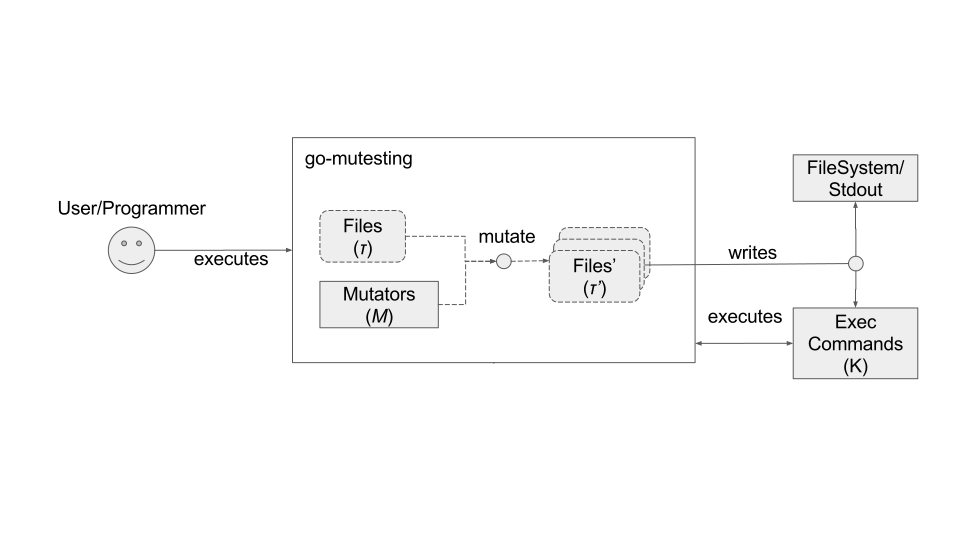
\includegraphics[width=1.1\textwidth]{images/go-mutesting-architecture.pdf}
\caption{Architecture of \textsc{go-mutesting}}
\label{fig:goMutestingArchitecture}
\end{figure}

Figure~\ref{fig:goMutestingArchitecture} depicts the main components of the \textsc{go-mutesting} framework. The user defines a set of files $\tau$ which should be mutated, and optionally a set of \texttt{exec commands} $\kappa$ which should be executed for each modification. Such modifications during mutation testing are called mutants. The framework applies its individual mutation operators called mutators $\mu$ on each file $\tau$, resulting in a set of mutated files $\tau'$ for each mutator-file pair. Each mutated file $\tau'$ is then written to the file system and executing the individual \texttt{exec commands} $\kappa$. After these executions are finished the framework prints the total number of mutants, the number of passing mutants and each failing mutant with their associated source code patches. We consider a mutant to pass in case the test suite failed for its mutation, which means that the mutant has therefore been killed.

Additional to the statistical output of mutants, \textsc{go-mutesting} calculates and outputs the mutation score. Which is a metric on how many mutants have been killed by the test suite and therefore states the quality of the test suite. The mutation score is calculated by dividing the number of passed mutants by the number of total mutants. If we had for example a total of eight mutants, where six are passing then the mutation score would be $6 / 8 = 0.75$. A score of $1.0$, which is most desirable, means that all mutants have been killed.

\section{Mutators}
\label{sec:goMutestingMutators}

The mutation operators of the \textsc{go-mutesting} framework are called mutators, and are used to introduce small deltas into the source files at hand. Mutators operate directly on the AST of a file and must offer two kinds of operations:
\begin{itemize}
\item The \texttt{Change} operation adapts the AST node at hand.
\item The \texttt{Reset} operation restores the original AST node.
\end{itemize}

Working directly on the AST has the advantage, that the introduced mutations are syntactical valid, i.e., compilable source code. Currently the following mutators are supported by the framework:

\begin{itemize}
\item The \texttt{if}-mutator replaces the body of an if-branch with a NOOP statement, which creates an empty usage for every identifier of the substituted body. This is necessary, since the programming language \textsc{Go} marks unused identifiers as syntactical errors.
\item The \texttt{else}-mutator replaces the body of an else-branch with a NOOP statement.
\item The \texttt{case}-mutator replaces the body of a case-clause with a NOOP statement.
\item The \texttt{remove-expression}-mutator modifies the binary logical operators \texttt{AND} and \texttt{OR}. The \texttt{AND} operator is mutated by replacing its left and right operands with the constant \texttt{true}. The \texttt{OR} operator is dealt with along the same lines by using the constant \texttt{false}. For instance, the binary logical expression \texttt{var1 \&\& var2} results in the two mutations \texttt{true \&\& var2} and \texttt{var1 \&\& true}.
\item The \texttt{remove-statement}-mutator modifies statements, such as assignments and the increment/decrement statement, by replacing them with a NOOP statement.
\end{itemize}

The above list of available mutators can easily be extended. A new mutator simply needs to provide the two mutation operations \texttt{Change} and \texttt{Reset}. Additionally, each mutator needs to be registered with the mutator registry of \textsc{go-mutesting} in order to be applied during mutation testing.

\section{Exec Commands}
\label{sec:goMutestingExecCommands}

\texttt{Exec commands} are used by \textsc{go-mutesting} to define the actions which should be taken for each individual mutant. Consider for instance a package with the following files: \texttt{LinkedList.go} and \texttt{LinkedList\_test.go}, where \texttt{LinkedList.go} is a linked list implementation and \texttt{LinkedList\_test.go} is the corresponding file for its tests. For each mutant that \textsc{go-mutesting} produces for the file \texttt{LinkedList.go}, a temporary file with the modifications of the mutant is written. Afterwards the specified \texttt{exec command} is called, executing the tests within \texttt{LinkedList\_test.go}.

A built-in \texttt{exec command} is provided by \textsc{go-mutesting}, which implements the following behavior:

\begin{enumerate}
\item Temporarily overwrite the original file, in our example \texttt{LinkedList.go}, with its mutated content.
\item Execute all tests of the package under test, which are in our example located in \texttt{LinkedList\_test.go}.
\item Restore the original file.
\item Report whether the mutant has been successfully killed.
\end{enumerate}

Customized \texttt{exec commands} can be specified as command line parameters of \textsc{go-mutesting}. Environment variables such as \texttt{MUTATE\_CHANGED} and \texttt{MUTATE\_ORIGINAL} are used to communicate the path of the original as well as the mutated file to the \texttt{exec command}. In order to report success or failure, the following exit codes need to be used by \texttt{exec commands}:
\begin{itemize}
\item Exit code 0 indicates that the mutant was killed, i.e., that the test led to a failed test after the mutation was applied.
\item Exit code 1 indicates that the mutant is alive, i.e., that this could be a flaw in the test suite or even in the implementation.
\item Exit code 2 indicates that the mutant was skipped, since other problems have been found such as compilation errors.
\item An exit code greater than 2 indicates that the mutant produced an unknown exit code, which might be a flaw in the \texttt{exec command}.
\end{itemize}

Two examples of customized \texttt{exec commands} are provided by \textsc{go-mutesting} at~\footnote{\url{https://github.com/zimmski/go-mutesting/tree/master/scripts/exec}}: \texttt{test-current-directory.sh} may be used to execute all tests of the current directory and \texttt{test-mutated-package.sh} to execute all tests originating from the specified package.
